\section{Approach}

% draw two pics, one is overview, describing a detail example. from candidate generation, focus entity identification, and a basic siamese structure. The other one is detailed network structure of our schema encoding.
In this section, we present our approach for solving complex KBQA.
First, we generate candidate query graphs by staged generation method (\secref{sec:candgen}).
Second, we measure the semantic similarities between the question and each query graph using deep neural networks (\secref{sec:rm}).
%Next we encode question and candidate query graph respectively. 
%More specifically, we use a bi-directianl RNN structure to represent question (\secref{sec:q-encoding}) and a complex embedding strategy is employed to encode a complex query graph (\secref{sec:schema-encoding}). Then we propose a cross attention mechanism to measure the similarity between a question and a query graph (\secref{sec:attention}).
Then we introduce an ensemble approach for entity linking enrichment (\secref{sec:ensemble}),
Finally, we discuss the prediction and parameter learning step of this task (\secref{sec:train}).
%Meanwhile, for finding improvements out of the neural network model, 
%we ultilize an ensemble approach to enrich the recall of entity linking method.


 
\section{Candidate Schema Generation}
\label{sec:candgen}

We propose a search algorithm to collect 
candidate schemas from training relation instances.
The intuition is that we first find suitable skeletons 
as a starting point, and then recursively add constraints on 
previous schemas, producing more specific candidate schemas.

%7 sentences introducing bfs
%1. recap
%As outlined in \secref{sec:problem}, a skeleton is a path of KB 
%predicates which connects target variables $x_1$ and $x_2$.
%2. basic: bfs
For each relation instance $(e_1, e_2)$, 
we use breadth-first search from both ends 
to find all suitable skeletons that connect them in KB.
%3. problem of connection
%Due to various predicates and popular entities existed, a relation 
%instance could be linked through a large number of different skeletons.
%4. what's meaningless rep.
%Most of natural language relations are short phrases, a skeleton 
%with too many predicates is meaningless, and is less likely 
%to be a suitable representation.
%5. solution to filter
We limit the maximum number of edges of the skeletons to be $\tau$.
%6. why use minimal coverage
The number of input relation instances
covered by a schema $S$ is called the {\em support} of $S$, or
$sup(S)$.
To ensure the quality of the retrieved skeleton, we also
require that $sup(S) \ge \gamma$. 
%Also note that we always focus on well-descriptive skeletons, 
%rather than some occasional paths covering only a few entity pairs.
%7. say in detail
%In formal, we define another threshold $cov$ as the minimum 
%percentage of entity pairs among all positive instances covered 
%by a skeleton.
% Comment: we could describe the searching process in detail, like Matt's style "more formally, blabla..."


%18 sentences: bfs basic, search space limit, budget, diversity
%1. general speak
After candidate skeletons are produced, we deploy depth-first search on
each skeleton to obtain more specific schemas.
At each step of the search, we attempt to add an edge to any one node
on the skeleton. An edge can be added if the support of the 
new schema is larger than $\gamma$. 
This process continues recursively until
no new schemas can be found.
%3-6: basic limit on schema constraints
%3. why need limitation
%The searching space is a tree structure which grows exponentially,
%making the exhaustive searching intractable on a huge knowlege base.
%4. how to fix the search size
Each additionl edge on a variable node acts like a constraint on the variable.
In practice, multiple constraints on the same variable seldom make sense. 
Therefore, we require that at most one edge is added to any node 
on the skeleton.
%5. the intuition behind
%As mentioned before, natural language relations are always short
%phrases, which gives us the point that it's less likely to infer
%a comfortable structure for a relation with multiple restriction 
%imposed on a single element, and our restriction just follows 
%this intuition.
%6. the effect of limitation
Consequently, the maximal depth of the searching tree is $\tau+1$.

%7-11: budget base (why, budget+prune, criteria, how to prune, diversity)
%7. why need budget
Unfortunately, each node in a skeleton may be attached hundreds of
different predicate in a large KB. The overall search space, though
bounded by the constant depth, is still large.
%8. introduce budget+pruning
Inspired by beam search algorithm\cite{ney1992data}, we introduce a fixed size 
priority queue to store the set of candidate schemas for each relation.
Our goal is to fill this queue (an operational budget) 
with relatively higher quality
schemas. We simply use the support of each schema on the input instances
as the quality or priority of the schema. The idea is that a better schema
should cover more instances. Also since as we attach more edges to the schema,
the support monotonically decreases, we can use this 
monotonicity property to prune the search
space. At each step of the search, we enumerate all the possible new schemas
(with one new edge) and insert the best among them to the priority queue if the
queue is not full. If the queue is full, we compare the support of the 
schema to be inserted with the worst schema on the queue. 
If the current schema is better than the worst schema on the queue, 
the worst schema is replaced and
the search continued from the current best schema. 
Otherwise, we prune the search space and backtrack.

%while pruning strategies will be used to reduce 
%searching space so that poor candidates could be ignored.
%9. what's the criteria
%To this end, we use the number of instances covered by 
%a schema as the criteria to approximately measure its quality.
%%10. explanation of the criteria
%The reason is two-fold: we aim to keep those descriptive schemas in 
%the output candidates, since we output a bunch of schemas instead
%of only a few, we don't need a rather precise quality measurement,
%the idea that better schemas cover more positive instances is
%reasonable enough for our task; 
%and the size of coverages would never increase when the search goes
%deeper, which leads to a simple but effective pruning strategy.
%
%11-15. formal describe
%Now we explain the searching step in formal.
%% [A simple pseudo code is available]
%The beginning state of the searching is one skeleton, we enumerate
%all the constraints which are allowed to add on, each constraint 
%maps to a more specific schema.
%Then new schemas are ranked over their coverages by descending order,
%and we sequentially continue recursive searching on those schemas.
%When the searching state comes to a new schema $s_0$, we keep this 
%schema if there has enough room to keep candidates; 
%otherwise, we pick the schema $s_1$ which has the smallest 
%coverage among all kept schemas and compare their coverage.
%If $s_0$ has a larger coverage, then $s_1$ is discarded, we keep 
%$s_0$ and search deeper; otherwise, the current schema $s_0$ is 
%pruned, and we backtrace the searching process immediately.
%Finally, the output candidates are those schemas been kept when
%the searching is over.

%16-18. diversity
Finally, we would like the generated set of candidate schemas
to be diverse and not all similar to each other.
%The diversity of output schemas plays an important rule in the 
%learning parts.
%If most candidates are the same and only differ from one or two 
%constraints, we are actually wasting budgets because it contains
%much redundant information.
We thus maintain multiple priority queues, one for each skeleton.
The size of each queue is proportional to the support of the corresponding
skeleton.



\begin{figure*}[ht]
	\centering
	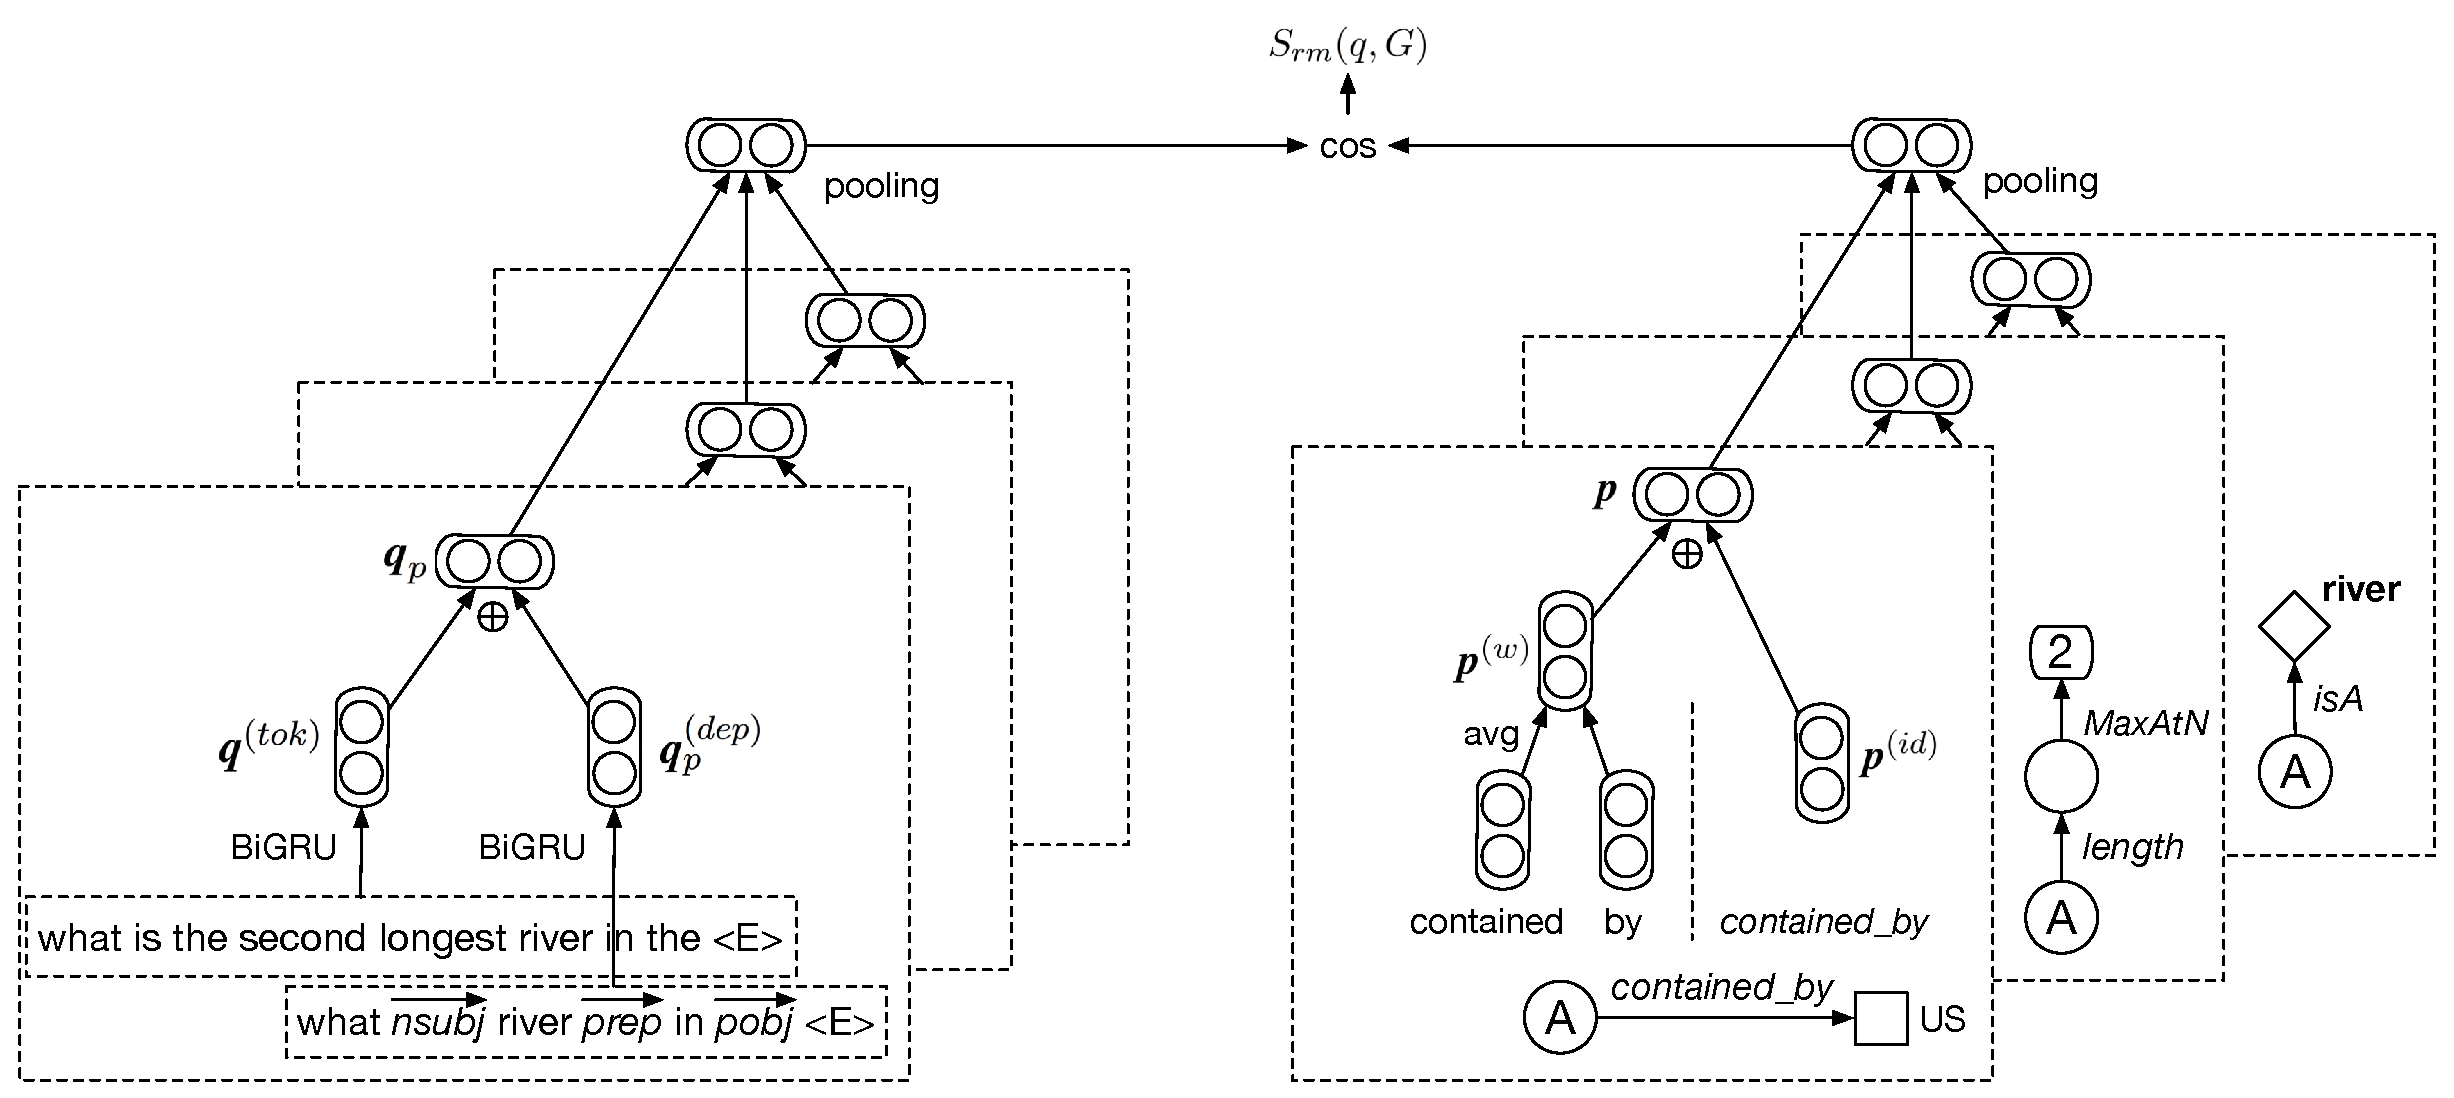
\epsfig{file=figures/overview.eps, angle=0, width=2.0\columnwidth}
	%\scalebox{0.3}{\includegraphics{overview.eps}}
	\caption{Overview of proposed semantic matching model.}
	\label{fig:nn}
\end{figure*}


\subsection{NN-based Semantic Matching Model}
\label{sec:rm}
%TODO: talk about the overview: cosine score, compact mode (merge then cos), two repr of questions and schema paths. Express them in the figure.
%TODO: 6 sents
%0. present the model in figure xxx: relation matching and entity linking
%1. the main part is RM: model as similarity task
%2. question side: sentential, syntactic
%3. path side: decomposition into parallel parts.
%4. each repr: relation sequence and name sequence.
%5. final score: combination of RM, EL and others.
%6. talk in detail.

The architecture of the proposed model is shown in \figref{fig:nn}.
%As a preprocessing step, we remove non-semantic information from both the question and the guery graph.
We first replace all entity (or time) mentions used in the query graph
by dummy tokens $\langle E \rangle$ (or $\langle Tm \rangle$).
%as changing ``United States'' to ``China'' doesn't affect the semantic meaning of
%our running example.
To encode the complex query structure,
we split it into predicate sequences starting from answer to focus nodes,
which we call \textit{semantic components}.
The predicate sequence doesn't include the information of focus nodes,
except for type constraints, where we append the focus type to the \textit{IsA} predicate,
resulting in the predicate sequence like \{\textit{IsA}, \textit{river}\}.
We introduce in detail the encoding methods for questions and predicate sequences,
and how to calculate the semantic similarity score.

%The propose neural network encodes both semantic components and questions
%into vector representation using sentential, syntactical and KB structural information.
%Finally the model merges vector representations of different components into 
%a the vector the entire graph,
%and calculate the semantic similarity of the query graph, given the question.



\subsubsection{Semantic Component Representation}
\label{sec:schema-encoding}

%TODO: Put this part into problem definition.
%After candidate generation, we obtain a set of candidate complex query graphs for each question $q$. A complex query graph $g$ can be regarded as a set of simple skeletons $(sk_1, sk_2, \dots, sk_m)$. We define a skeleton $sk$ is a predicate path starting from a fixed node to the target answer. The fixed starting node can be an entity, a type, a number, datetime or an ordinal value. Together with predicate, we call them ``items''. Thus we denote $sk = (it_1, it_2, \dots, it_l)$ (Note that this sequence has an order from starting point to target answer). In the case of \figref{fig:overview}, the candidate query graph in the right side can be splited into three skeletons, which start from ``entity:China'', ``type:River'' and ``ordinal$\_$value:$2$'' respectively. 

%In the part of relation matching, we need to encode the query graph.
%To encode the query graph, we first decompose the graph into semantic aspects.
%The semantic aspect is defined as one path in the query graph,
%which starts from the answer node and ends with a leaf node (candidate entities, types, times, ordinals).
%As the example shown in \figref{xxx},
%the candidate graph is decomposed into 3 semantic aspects which provide the following parallel clues:
%``the answer is in China'',
%``the answer is a river'', 
%``the answer ranks second by descending order of length''.
%The whole query graph represents the combination of clues, representing a complex semantics.



To encode a semantic component $p$, we take the sequence of both predicate ids
and predicate names into consideration.
As the example shown in \figref{fig:nn}, the id sequence of the first semantic component
is \{\textit{contained\_by}\}, 
and the predicate word sequence is the concatenation of canonical names for each predicate,
that is \{``contained'', ``by''\}.
%We use both id and labels in the knowlege base to encode each semantic aspect.
%Each aspect repred by a sequence of KB predicates and types along the path.
%Leave entities, times and ordinal numbers out. (don't care the detail time, number or entities)
%Sequence at different granularities.
%word sequence of the path: $p^{(w)} = \{p_1^{(w)}, \dots, p_n^{(w)}\}$.
%id sequence of the path: $p^{(id)} = \{p_1^{(id)}, \dots, p_m^{(id)}\}$.
%(from type.object.name relation.)

%Different methods to encode the path representation given the sequences.

Given the word sequence $\{p_1^{(w)}, \dots, p_n^{(w)}\}$, %we use word embedding matrix to transform words into vectors.
we first use a word embedding matrix $E_w \in \mathbb{R}^{|V_w| \times d}$ to convert 
the original sequence into word embeddings $\{\bi{p}_1^{(w)}, \dots, \bi{p}_n^{(w)}\}$,
where $|V_w|$ denotes the vocabulary size of natural language words,
and $d$ denotes the embedding dimension.
%TODO: talk later
%The word embedding matrix is initialized by publicly available pre-trained results, 
%such as Word2vec~\cite{mikolov2013} and GloVe~\cite{xxx}. 
Then we represent the word sequence using word averaging:
%Then we encode the whole sequence in continuous bag-of-words 
%\textbf{Bag-of-Words}:
$\bi{p}^{(w)} = \frac{1}{n} \sum_{i}{\bi{p}_i^{(w)}}$.

%\textbf{Recurrent-Words}: We use GRU~\cite{xx} as the recurrent cell.
%The sequence of word vectors are fed into a bidirectional GRU layer,
%and the repr is the concatenation between the last forward and backward hidden states,
%$\bi{p}^{(w)} = [\overrightarrow{\bi{h}}_n^{(w)};\overleftarrow{\bi{h}}_1^{(w)}]$

For the id sequence $\{p_1^{(id)}, \dots, p_m^{(id)}\}$,
%similarly, we have \textbf{Bag-of-Ids} and \textbf{Recurrent-Ids}
%for encoding the id sequence via another id embedding matrix
%$E_{id} \in \mathbb{R}^{|V_{id} \times d|}$.
we simply take it as a whole unit, and directly translate it into vector representation
using the embedding matrix $E_p \in \mathbb{R}^{|V_p \times d|}$ at path level,
where $|V_p|$ is the vocabulary size of predicate sequences.
There are two reasons for using such path embedding:
1) the length of id sequence is not larger than two, based on our generation method;
2) the number of distinct predicate sequences is roughly the same as the number of distinct predicates.
%Considering that the length of id sequence is restricted (mostly no longer than 2 hops),
%we propose the third method \textbf{Whole-Path}, 
%as it takes the id sequence as a whole unit, and directly transforms it into vector representation,
%by using the embedding matrix at path level,
%$E_p \in \mathbb{R}^{|V_p \times d|}$.
We get the final vector of the semantic component by element-wise addition:
$\bi{p} = \bi{p}^{(w)} + \bi{p}^{(id)}$.




%Now we describe in detail how to obtain the skeleton representation $\bi{sk}$ and further represent a complex query graph $g$ into $\bi{g} = (\bi{sk}_1, \bi{sk}_2, \dots, \bi{sk}_m)$. 
%
%%1. item encoding
%Firstly, we represent each component (item) of a skeleton into hidden vectors. For entity, type and predicate, we use their names in KB as text infomation and thus employ a bi-GRU network to encode the items just as we do in question encoding (\secref{sec:q-encoding}). For example, the name of entity ``China'' in \figref{fig:overview} is \textit{``People's Republic of China''} and we regard it as a word sequence [``people'', ``republic'', ``of'', ``China'']. After embedding lookup, the sequence of word embeddings are fed into bi-GRU, resulting a sequence of hidden vectors $[\overrightarrow{\bi{h}_i};\overleftarrow{\bi{h}_i}]$. Then we average them to obtain the item representation $\bi{it}$.
%
%\begin{equation}
%\label{eqn:item}
%\begin{aligned}
%& \bi{it} & = & \frac{1}{N}\sum_{i}[\overrightarrow{\bi{h}_i};\overleftarrow{\bi{h}_i}]\\
%\end{aligned}
%\end{equation}
%\noindent
%where $N$ is the number of words in that name.
%For number, datetime and ordinal value, we add three special placeholders in word embedding vocabulary and initialize them randomly. Thus, these three items are represented directly through embedding lookup. 
%
%%2. skeleton representation
%
%Then, we represent a skeleton $\bi{sk}$ as a dynamic combination of its item representations $\bi{it}_i$ shown in \figref{fig:overview} (right side). Since the items of a skeleton also form into a sequence in order, we use another bi-GRU to encode item sequence.
%
%Up to now, we have obtained the representation of query graph $\bi{g}$ consisting of a set of skeletion representations $(\bi{sk}_1, \bi{sk}_2, \dots, \bi{sk}_m)$.



\subsubsection{Question Representation}
\label{sec:qw-repr}

%Before encoding the question,
%%As a preprocess step, 
%we replace all entity mentions in the current query by a dummy token $\langle E \rangle$,
%and all time mentions by $\langle Tm \rangle$.
%The running example will be transformed into ``What is the second longest river in $\langle E \rangle$ ?''
%given the candidate query in \figref{xxx}.
%Therefore, two questions share the same semantic representation,
%if they have the same structure, but only differ in focus entities or times.


%We aim at finding the association between the question and different semantic components.
%Now we encode the question into vector representation.
%Given a candidate query structure with multiple focus nodes,
%our goal is to find the association between the question and different semantic aspects.
We encode the question in both global and local level,
which captures the semantic information with respect to each component $p$.

The global information takes the token sequence as the input.
We use the same word embedding matrix $E_w$ to convert the token sequence into vectors
$\{\bi{q}_1^{(w)}, \dots, \bi{q}_n^{(w)}\}$.
Then we encode the token sequence by applying bidirectional GRU network~\cite{cho2014properties}.
%\textbf{Recurrent-Words}: We use GRU~\cite{xx} as the recurrent cell.
%The sequence of word vectors are fed into a bidirectional GRU layer,
The representation of the token sequence is the concatenation
of the last forward and backward hidden states through the BiGRU layer,
$\bi{q}^{(tok)} = [\overleftarrow{\bi{h}}_1^{(w)};\overrightarrow{\bi{h}}_n^{(w)}]$.

%Then we feed the word embeddings into the bidirectional GRU layer
%for capturing long-distance dependencies of the sentence.
%%TODO: positional embedding
%Similarly, we concatenate the last forward and backward state to produce the embedding representation
%at token level $\bi{q}_p^{(tok)}$.
%%at token level: $\bi{q}^{(tok)} = [\overrightarrow{\bi{h}}_n^{(w)};\overleftarrow{\bi{h}}_1^{(w)}]$

To encode the question at local level,
%we look for relevant semantic clues with respect to the particular semantic component $p$.
%That is, given a path, try to find salient evidence sequence, and remove irrelevant words.
%discovering   the answer 
%For example in \figref{fig:nn}, the semantic meaning of \textit{contained\_by}
%is aligned to the sub-question ``What is in $\langle E \rangle$''.
%To this end,
we leverage dependency parsing to represent
long-range dependencies between the answer and the focus node in $p$.
%For this goal, we use dependency parsing as the source to guide us find the meaningful words through syntactic evidences.
Since the answer is denoted by the wh- word in the question,
we extract the dependency path from the answer node to the focus mention in the question.
%The path is unique since the dependency parsing result is a tree.
Similar with \citet{xu2016question},
we treat the path as the concatenation of words and dependency labels with directions.
For example, the dependency path between ``what'' and ``United States'' is
\{what, $\overrightarrow{nsubj}$, is, $\overrightarrow{prep}$, in, $\overrightarrow{pobj}$, $\langle E \rangle$\}.
%Given the parsing tree of the question,
%we extract the dependency path from the answer node (wh- words in the question) to the focus mention of the semantic aspect.
%For the first aspect in \figref{xxx}, the dependency path between ``what'' and ``China''
%is \{what, \textit{xxx-1}, is , \textit{yyy}, in \textit{zzz}, $\langle E \rangle$\},
%where focus word ``China'' is also replaced by $\langle E \rangle$.
%The path is unique since the parsing result is a tree, and the path is a combination
%of both related tokens and dependency arcs.
%We use \textit{xxx-1} for representing the reverse direction of the arc \textit{xxx}.
We apply another bidirectional GRU layer to produce the vector representation at dependency level
$\bi{q}_p^{(dep)}$, capturing both syntactic features and local semantic features.
%TODO: draw a figure for showing the two GRUs, one for sentential and one for syntactical.
%Fianlly, as illustrated in \figref{xxx}
%With the guide of semantic component $p$,
Finally we combine global and local representation by element-wise addition,
returning the representation of the question with respect to the semantic component, 
$\bi{q}_p = \bi{q}^{(tok)} + \bi{q}_p^{(dep)}$.
%TODO: try FC here???????




%Before the step of cross-attention, we encode the input questions as the distributional
%representation of each word in it.
%Specifically, the input question $q$ is expressed as the word sequence $q=(w_1, w_2, \dots, w_n)$,
%where $w_i$ denotes the $i$-th word.
%%TODO: trick of E and Tm
%We first use a word embedding matrix $E_w \in \mathbb{R}^{|V_w| \times d}$ to convert 
%the original sequence into word embeddings $\bi{q}=(\bi{w}_1, \bi{w}_2, \dots, \bi{w}_n)$,
%where $|V_w|$ denotes the vocablary size of natural language words,
%and $d$ denotes the embedding dimenson.
%The word embedding matrix is initialized by publicly available pre-trained results, 
%such as Word2vec~\cite{mikolov2013} and GloVe~\cite{xxx}. 

%In the next step, we feed the word embeddings into a bidirectional Gated Recurrent Unit (GRU)~\cite{xxx} networks.
%As a brief introduction, GRU is capable of effectively maintaining the long-distance dependency in many NLP tasks.
%Given $\bi{x}_t$ as the input of time step $t$ of RNN, and $\bi{h}_{t-1}$ as the hidden state at time stamp $t-1$,
%GRU calculates the current hidden state $\bi{h}_t$ through gated units, described in \eqnref{eqn:gru}:
%
%\begin{equation}
%  \label{eqn:gru}
%  \begin{aligned}
%    & \bi{r}_t & = & \sigma(\bi{W}_r\bi{x}_t+\bi{U}_r\bi{h}_{t-1}), \\
%    & \bi{z}_t & = & \sigma(\bi{W}_z\bi{x}_t+\bi{U}_z\bi{h}_{t-1}), \\
%    & \tilde{\bi{h}}_t & = &\mbox{tanh}(\bi{W}_h\bi{x}_t+\bi{U}_h(\bi{r}_t\cdot\bi{h}_{t-1})), \\
%    & \bi{h}_t & = & (1-\bi{z}_t)\cdot\bi{h}_{t-1}+\bi{z}_t\cdot\tilde{\bi{h}}_t. \\
%  \end{aligned}
%\end{equation}
%
%\noindent
%In the case of GRU, the vector $\bi{r}_t$ is the output of the \textit{reset gate},
%determining how much information of the last state $\bi{h}_{t-1}$ is ignored
%in the computation of the candidate state $\tilde{\bi{h}}_t$.
%The vector $\bi{z}_t$ is the output of the \textit{update gate}, which controls the interpolation 
%between the last state $\bi{h}_{t-1}$ and the candidate state $\tilde{\bi{h}}_t$.
%
%For encoding the input question, we employ the bidirectional GRU network, which consists a
%forward network and a backward network encoding in the reverse order.
%Taking the word embedding sequence $(\bi{w}_1, \dots, \bi{w}_n)$ as input,
%we get the forward hidden sequence
%$(\overrightarrow{\bi{h}_1}, \overrightarrow{\bi{h}_2}, \dots, \overrightarrow{\bi{h}_n})$ 
%as well as the backward one
%$(\overleftarrow{\bi{h}_1}, \overleftarrow{\bi{h}_2}, \dots, \overleftarrow{\bi{h}_n})$.
%We concatnate the forward hidden state of each word with corresponding backward hidden state,
%resulting in the distributional representation $\bi{h}^{(w)}_i = [\overrightarrow{\bi{h}_i};\overleftarrow{\bi{h}_i}]$.
%Thus, we obtain the representation of each word in the question, and each hidden state
%encodes the information from both before and after the corresponding word.





\subsubsection{Semantic Similarity Calculation}

%Now we define the similarity function between the question $q$ 
Given the query graph with multiple semantic components, $G = \{p^{(1)}, \dots, p^{(N)}\}$,
now all its semantic components have been projected into a common vector space,
representing hidden features in different aspects.
%Inspired by the architecture of CNN,
%common vector for sub.
%where features of a whole image is determined by the      in some region
%Each component represents partial semantic information of the query graph.
%map to a common vector space
%part of semantics
%inspired by CNN, the repr of determined by whether a subregion has such feature
We apply max pooling over the hidden vectors of semantic components,
and get the compositional semantic representation of the entire query graph.
Similarly, we perform max pooling for the question vectors 
with respect to each semantic component.
Finally, we compute the semantic similarity score between the graph and question:
\begin{equation}
S_{sem}(q, G) = cos(\max_{i}{\bi{p}^{(i)}}, \max_{i}{\bi{q}_p^{(i)}}).
\end{equation}

Based on this framework, our proposed method ensures
the vector spaces of the question and the entire query graph are comparable,
and captures complementary semantic features from different parts of the query graph.
It's worth mentioning that the semantic matching model 
is agnostic to the candidate generation method of the query graphs,
hence it can be applied to the other existing semantic parsing frameworks.


\subsection{Entity Linking Enrichment}
\label{sec:ensemble}

The S-MART linker is a black box for our system,
which is not extendable and tend to produce high precision but low recall linking results.
To seek a better balance at entity linking,
we propose an ensemble approach to enrich linking results.
We first build a large lexicon by collecting all (mention, entity) pairs from
article titles, anchor texts, redirects and disambiguation pages of Wikipedia.
Each pair is associated with statistical features, such as linking probability,
letter-tri-gram jaccard similarity and popularity of the entity in Wikipedia.
For the pairs found in S-MART results, we take the above features as the input
to a 2-layer linear regression model fitting their linking scores.
Thus we learn a pseudo linking score for every pair in the lexicon,
and for each question, we pick top-$K$ highest pairs to enrich S-MART linking results,
where $K$ is a hyperparameter.
%In addition, we add two more linking features,
%each indicating whether a (mention, entity) pair comes from S-MART or our lexicon.


\subsection{Training and Prediction}
\label{sec:train}


To predict the best query graph from candidates,
we calculate the overall association score $S(q, G)$ between the question $q$ and each candidate $G$,
which is the weighted sum of features over entity linking, semantic matching and structural level.
\tabref{tab:feature} lists the detail features.



%\begin{itemize}
%\item Semantic similarity score $S_{sem}(q, G)$;
%\item Sum of S-MART (or pseudo) linking scores of all entities in $G$;
%\item Sum of binary features over all entities,
%      each indicating whether the entity comes from S-MART or enriched lexicon.
%\item Number of each kind of constraints (entity, type, time, ordinal) applied in $G$;
%\item Binary features, each indicating whether a kind of constraints is applied in $G$ or not;
%\item Binary feature indicating whether the main path is 1-hop;
%\item One-hot vector indicating the number of answers queried by $G$.
%\end{itemize}
%TODO: change to table style (Berant or other 17/18 papers)

%3. optimization
%
%loss pick
%separately measure: entity linking and relation matching
%max function: F1\_r = ...
%generate candidates by particular F1 sequence
%joint style, 
%
%final schema: feature cominbation
%entity linking score: enhancement
%
%optm: random sample 20 negatives (set threshold = 0.1)
%lower them.
%
%max margin
%
%rm f1, el f1, full f1
During training step, we adopt hinge loss to maximize the margin
between positive graphs $G^+$ and negative graphs $G^-$:
\begin{equation}
\label{eqn:maxpool}
loss = max\{0, \lambda - S(q, G^+) + S(q, G^-)\}.
\end{equation}
For each question, we pick a candidate graph as positive data,
if the $F_1$ score of its answer is larger than a threshold (set to 0.1 in our work).
We randomly sample 20 negative graphs $G^-$ from the candidate set
whose $F_1$ is lower than the corresponding $G^+$.
%TODO: Tricks

\begin{table}[ht]
    \small
    \centering
    \begin{tabular}{|c|l|}
        \hline
        \textbf{Category}    & \textbf{Description}   \\
        \hline
        Entity  & Sum of S-MART scores of all entities; \\
                & Number of entities from S-MART; \\
                & Number of entities from enriched lexicon; \\
        \hline
        Semantics & Semantic similarity score $S_{sem}(q, G)$; \\
        \hline
        Structural  &  Number of each kind of constraints in $G$; \\
                    &  Whether a kind of constraints is used in $G$; \\
                    &  Whether the main path is one-hop; \\
                    &  Number of output answers. \\
        \hline
    \end{tabular}
    \caption{Full set of features.}
    \label{tab:feature}
\end{table}

%TODO: bao, yih: we don't need pre-train



%\subsection{Attention Mechanism}
%\label{sec:attention}
%
%Attention mechanisms \cite{bahdanau2014neural,luong2015effective} have become an integral part of sequence modeling and transduction models in various nlp tasks, allowing better understanding sequential data. In this paper, we introduce a cross-attention mechanism between question and query graph, aiming to better justify thier compatibility.
%
%Our cross-attention mechanism consists of two parts: query graph towards question part and question towards query graph part. Our goal is to find the best query graph from the candidate set. When we look at a question $\bi{q} = (\bi{q}_1, \bi{q}_2, \dots, \bi{q}_n)$ and a candidate query graph $\bi{g} = (\bi{sk}_1, \bi{sk}_2, \dots, \bi{sk}_m)$, we have to judge which parts of the query graph are more related to the question, since each skeleton of a graph describes one semantic aspect of the question. Besides, when we look at the query graph, we will reread the question to find out which words are more focused. Hao et al., \cite{hao2017end} also propose a cross-attention mechanism, aiming to select the best answer towards a question. However, their method does not calculate the attention values on both sides simultaneously, instead they do it in two steps and use an average of word representations in question to guide the attention of answer aspects. 
%
%\begin{figure*}
%	\centering
%	\epsfig{file=figures/attention.eps, angle=0, width=1.2\columnwidth}
%	%\scalebox{0.5}{\includegraphics{figures/attention.eps}}
%	\caption{Cross-attention architecture between question and query graph.}
%	\label{fig:attention}
%\end{figure*}
%
%Inspired by ABCNN \cite{yin2015abcnn}, we propose a attention matrix $\bi{E}_{att}$  (\figref{fig:attention}), where the attention values of row $i$ denote the attention distribution of the $i$-th word in the question with respect to the query graph, and the attention values of column $j$ denote the attention distribution of the $j$-th skeleton in the query graph with respect to the question. Then we represents the whole question $\bi{q}$ and query graph $\bi{g}$ as follows. 
%
%
%
%
%\begin{equation}
%\label{eqn:att-q}
%\begin{aligned}
%& \bi{q} & = & \sum_{i}(\sum_{j}{\bi{E}_{att}}_{ij}) \times \bi{q}_i\\
%\end{aligned}
%\end{equation}
%\noindent
%
%\begin{equation}
%\label{eqn:att-g}
%\begin{aligned}
%& \bi{g} & = & \sum_{j}(\sum_{i}{\bi{E}_{att}}_{ij}) \times \bi{sk}_j\\
%\end{aligned}
%\end{equation}
%\noindent
%
%In the end, we use a fully connected layer to get a similarity score between $\bi{q}$ and $\bi{g}$.
%
%
%
%\subsection{Training and Prediction}
%\label{sec:training}
